\documentclass[a4paper,twoside]{article}

% baseline packages
\usepackage[top=2.5cm, bottom=2.5cm, left=2.5cm, right=2.5cm]{geometry}
\usepackage{graphicx}
\DeclareGraphicsExtensions{.pdf,.png,.jpg,.mps,.eps,.ps}
\graphicspath{{figures/}{.}}
\usepackage[numbers,sort&compress,super,comma]{natbib}
\usepackage[table]{xcolor}
\usepackage{booktabs} % professional-quality tables
\usepackage{multirow}
\usepackage{enumitem}
\usepackage{hyperref} % for clickable links
\hypersetup{
    colorlinks = true,
    citecolor = .,
    linkcolor = .
    }
\usepackage{url}

% make it pretty
\usepackage{microtype} % improve typography
\usepackage[T1]{fontenc} % T1 encoding helps proper hyphenation and text rendering in European languages (without this OT1 is default)
\usepackage[default]{lato} % make Lato the default font
\usepackage{fancyhdr}
\usepackage{titling}

\pagestyle{fancy}

% Horizontal line settings
\renewcommand{\headrulewidth}{2pt}
\renewcommand{\footrulewidth}{1pt}

% Header and footer setup
\fancyhead{} % clear all fields
\fancyhead[C]{\emph{internal notes}}
\fancyhead[L]{Park et. al.}
\fancyfoot[C]{\thepage}

% Title setup with affiliations
\pretitle{\begin{center}\LARGE}
\posttitle{\end{center}}
\preauthor{\begin{center}
\large \lineskip 0.5em}
\postauthor{\par\end{center}
\begin{center}
\textit{
$^1$Champalimaud Centre for the Unknown, Champalimaud Foundation, Lisbon, Portugal
}
%\\
%$^\ast$corresponding author, \url{memming.park@research.fchampalimaud.org}
\end{center}}

\title{Deriving measures of dissimilarity between systems}
\author{
I.~Memming~Park$^{1}$ and
Abel S\'agodi$^{1}$
}
\date{\today}

% math & font packages
\usepackage[fleqn]{amsmath} % align equations left
\usepackage{amssymb}
\usepackage{mathtools} % \DeclarePairedDelimiter
\usepackage{bm} % bold greek

% cosmetics
\usepackage{letltxmacro}
\LetLtxMacro{\originaleqref}{\eqref}
\renewcommand{\eqref}{Eq.~\originaleqref}

%%%%%%%%%%%%%%%%%%%%%%%%%%%%%%%%%%%%%%%%%%%%%%%%%%%%%%%%
% bold vectors for each alphabet vx
\usepackage{forloop}
\newcommand{\defvec}[1]{\expandafter\newcommand\csname v#1\endcsname{{\mathbf{#1}}}}
\newcounter{ct}
\forLoop{1}{26}{ct}{
    \edef\letter{\alph{ct}}
    \expandafter\defvec\letter
}

% captial \vA
\forLoop{1}{26}{ct}{
    \edef\letter{\Alph{ct}}
    \expandafter\defvec\letter
}

%%%%%%%%%%%%%%%%%%%%%%%%%%%%%%%%%%%%%%%%%%%%%%%%%%%%%%%%
% Automatically make all greek letters bold by prepending 'v'
\usepackage{expl3}

\ExplSyntaxOn
% Define a sequence of Greek letters
\cs_new:Nn \define_bold_greek:
 {
  \seq_map_inline:Nn \g_greek_letters_seq
   {
    \cs_new:cpn { v##1 } { \bm { \csname ##1 \endcsname } }
   }
 }

% Initialize the sequence of Greek letters
\seq_new:N \g_greek_letters_seq
\seq_set_split:Nnn \g_greek_letters_seq { , }
 {
  alpha,beta,gamma,delta,epsilon,zeta,eta,theta,iota,kappa,lambda,
  mu,nu,xi,pi,rho,sigma,tau,upsilon,phi,chi,psi,omega,
  Delta
 }

% Call the function to define bold Greek macros
\define_bold_greek:
\ExplSyntaxOff
%%%%%%%%%%%%%%%%%%%%%%%%%%%%%%%%%%%%%%%%%%%%%%%%%%%%%%%%

% Math commands
\DeclareMathOperator{\diag}{diag}
\DeclareMathOperator{\vecOp}{\rm vec} % vec operator
\DeclareMathOperator*{\tr}{tr} % trace
\DeclareMathOperator*{\argmax}{\rm argmax}
\DeclareMathOperator*{\argmin}{\rm argmin}
\DeclareMathOperator*{\var}{var}
\DeclareMathOperator*{\cov}{cov}
\newcommand{\divv}{\ensuremath{\mathbb{D}}}
\newcommand{\KL}[2]{\divv_{\text{KL}}\!\left({#1}\middle\lvert\middle\rvert\,{#2}\right)}
\newcommand{\IMPdivv}[3]{\divv_{\text{IMP}}\!\left({#1}\middle\lvert\middle\rvert\,{#2}\,;{#3}\right)}
\newcommand{\dis}{\ensuremath{\mathcal{D}}}

\DeclarePairedDelimiter{\abs}{\lvert}{\rvert}
\DeclarePairedDelimiter{\norm}{\lVert}{\rVert}

\DeclareMathOperator*{\E}{\rm E} % expectation
\newcommand{\inv}{^{-1}}
\newcommand{\dm}[1]{\ensuremath{\mathrm{d}{#1}}} % dx dy dz dmu
\newcommand{\RN}[2]{\frac{\dm{#1}}{\dm{#2}}} % (Radon-Nikodym) derivative
\newcommand{\PD}[2]{\frac{\partial #1}{\partial #2}} % partial derivative

\newcommand{\field}[1]{\ensuremath{\mathbb{#1}}}
\newcommand{\reals}{\field{R}}
\newcommand{\complex}{\field{C}}
\newcommand{\integers}{\field{Z}}
\newcommand{\naturalNumbers}{\field{N}}
\newcommand{\trp}{{^\top}} % transpose
\newcommand{\identity}{\ensuremath{\mathbb{I}}}
\newcommand{\ones}{\ensuremath{\mathbf{1}}}
\newcommand{\indicator}[1]{\mathbf{1}_{#1}} % indicator function
\newcommand{\stateSpace}{\reals^n}
\newcommand{\DF}{\nabla_{\vx}\vf} %\newcommand{\DF}{\mathcal{D}\vf}

%%%%%%%%%%%%%%%%%%%%%%%%%%%%%%%%%%%%%%%%%%%%%%%%%%%%%%%%
\definecolor{mpcolor}{rgb}{1, 0.1, 0.59}
\newcommand{\TODO}[1]{(\textbf{TODO:\ }\textcolor{mpcolor}{#1})}

\definecolor{c:adjointidx}{rgb}{0.15,0.55,0.7}
\definecolor{c:time}{rgb}{0.50,0.12,0.7}
\newcommand{\homeo}{\vh}
\newcommand{\invhomeo}{\homeo\inv}

%%%%%%%%%%%%%%%%%%%%%%%%%%%%%%%%%%%%%%%%%%%%%%%%%%%%%%%%
\begin{document}
\maketitle
\thispagestyle{fancy}

\section{Background}
Let us consider two autonomous dynamical systems defined on the same space:
\begin{align}
    \begin{cases}
    \dot{\vx} &= \vf(\vx)
    \\
    \dot{\vx} &= \vg(\vx)
    \end{cases}
\end{align}

If the two systems are topologically equivalent, there exists a homeomorphism $\homeo$ that maps orbits of one system to the other.
 Furthermore, if the flow of time is preserved, they are topologically conjugate.

Let $\homeo$ be a diffeomorphism (which means $\homeo$ is a smooth homeomorphism).
\begin{align}
    \vy &= \homeo(\vx)
    \\
    \dot{\vy} &=
	\nabla\homeo(\vx)\dot{\vx}
    =
	\nabla\homeo(\vx) \vf(\vx)
    =
	\nabla\homeo(\invhomeo(\vy)) \vf(\invhomeo(\vy))
	\label{eq:distortion:homeo}
    \\
    \dot{\vx} &= \nabla\homeo(\vx)\inv \dot{\vy}
\end{align}
where $\nabla$ is the Jacobian operator, and $\nabla\homeo(\cdot)$ is a matrix function.
The two systems are \emph{smoothly equivalent} if
\begin{align}
    \dot{\vx} &= \nabla\homeo(\vx)\inv \vg(\homeo(\vx)) = \vf(\vx)
\end{align}

Recall that a vector field is called \emph{structurally stable} if all vector fields in its neighborhood (in $C^1$ topology), are topologically conjugate to the given vector field~\cite{Chicone2006}.

\section{Distortions, Perturbations, Deformation, or Imperfections}
Let us consider two kinds of distortions.

\subsection{Additive Perturbation}
First we have additive vector field perturbation by $\vDelta(\cdot)$.
\begin{align}
    \dot{\vx} &= \vf(\vx) + \vDelta(\vx)
\end{align}
For a finite time horizon $T$ and assuming a Lipschitz bound $L$ for $\vf$ in the relevant domain, a uniform bound on $\norm{\vDelta(\cdot)}$, we can bound the trajectory deviation from the unperturbed system.
By Gr\"onwall inequality\cite{Howard2025}:
\begin{align}
    \norm{
	\phi(\vf, \vx_0, t)
	-
	\phi(\vf + \vDelta, \vx_0, t)
    }
    &\leq
	e^{Lt} \int_0^t e^{-Ls} \norm{\vDelta(s)} \,\mathrm{d}s
\\
    &\leq
	\left(\sup_s \norm{\vDelta(s)}\right) e^{Lt} \int_0^t e^{-Ls} \,\mathrm{d}s
    =
	\left(\sup_s \norm{\vDelta(s)}\right) \frac{1}{L} (e^{Lt} - 1)
\end{align}
for any norm $\norm{\cdot}$ and where $\phi$ denotes the trajectory (solution to the initial value problem).
Thus, for small additive perturbation, the trajectories are robust as long as the Lipschitz constant is not too wild.

Note that additive perturbation can change the stability structure such that topological conjugacy and equivalence are broken.

\subsection{Homeomorphic/Diffeomorphic Perturbation}
The second kind of distortion is a deformation with a diffeomorphism $\homeo$.
The perturbed system is given by \eqref{eq:distortion:homeo}.
As it preserves the topological structure of the system, it behaves \emph{qualitatively} the same, and they share the corresponding asymptotic dynamcal structures such as fixed points, limit cycles, and invariant manifolds.
However, depending on the ``complexity'' of $\homeo$, it may distort the space (and speed) more or less which can be quantified locally by how much it stretches and shrinks in various directions.
\begin{align}
    \dot{\vx} &= \vf(\vx)
    \\
    \dot{\vy} &= \vg(\vy)
	= \nabla\homeo(\invhomeo(\vy)) \vf(\invhomeo(\vy))
    % = \nabla\homeo(\vx) \vf(\vx)
\end{align}
If the homeomorphism is close to identity, it makes sense to relate it to the induced additive perturbation.
If we take the difference of vector field, we get
\begin{align}
    \vDelta_h(\vx) &\coloneqq \vf(\vx) - \vg(\vx) =
	\vf(\vx) -
	\nabla\homeo(\invhomeo(\vx)) \vf(\invhomeo(\vx))
\end{align}

\subsection{Affine transformation}
We treat systems equivalent if an invertible affine transformation maps one system to another.

\section{Dissimilarity}
Given a source and target system pair and distribution over trajectories, we would like to measure their dissimilarity.
First, we consider a point-wise measure of dissimilarity that measures the required additive perturbations and diffeomorphic deformations to apply to the source system to obtain the target system.

\subsection{Imperfection}
Mapping the asymptotic structure of the two systems to align is a preferable distortion, however, since diffeomorphism is limited to smoothly equivalent systems, we need the additive perturbation to take into account the slack.
Therefore, we first consider the minimum additive perturbation to achieve topological conjugacy.
\begin{align}
    \vDelta_1(\vx) &= \argmin \norm{\tilde \vDelta}
    \label{eq:d1:min}
    \\
    & \text{s.t.} \quad
    \vf(\vx) + \tilde \vDelta(\vx)
    \overset{\text{t.c.}}{\sim}
    \vg(\vx)
    \label{eq:d1:tc}
\end{align}

We identify this gap $\vDelta_1$ as the \emph{imperfection}.

\subsection{First-order bound and the Pareto frontier}
Let $\homeo^\ast$ be a diffeomorphism that can be used for achieving the smooth conjugacy in \eqref{eq:d1:tc}.
Now, we want to consider the complexity of $\homeo$ and trade-off with additive perturbation.
For this, we will do a first-order perturbation analysis.

To link the complexity of diffeomorphism to the magnitude of additive perturbation, we seek to find the equivalence up to first order of the vector field corresponding to the diffeomorphism.
That is, we seek to find $\vDelta(\vx)$ that maintains the topological conjugacy,
\begin{align}
    \dot\vx = \vf(\vx) + \epsilon \vDelta(\vx)
    \overset{\text{t.c.}}{\sim}
    \vg(\vx)
    \label{eq:pareto:tc}
\end{align}
where $\epsilon > 0$.

We assume an Ansatz for the diffeomorphism, under the assumption that it is close to identity:
\begin{align}\label{eq:h:ansatz}
    \vy &= \homeo(\vx) = \vx + \epsilon \tilde\homeo(\vx) + O(\epsilon^2)
\end{align}
Note that from \eqref{eq:h:ansatz}, we have
\begin{align}
    \nabla\vh(\vx) &= \identity + \epsilon\nabla\tilde\vh(\vx) + O(\epsilon^2)
\end{align}
By taking the time derivative of \eqref{eq:h:ansatz}, we get
\begin{align}
    \dot{\vy} &= \dot{\vx} + \epsilon \nabla\tilde\homeo(\vx)\dot{\vx} + O(\epsilon^2)
    \\
    &=
	\vf(\vx) + \epsilon \vDelta(\vx)
	+ \epsilon \nabla\tilde\homeo(\vx)
	\left(
	    \vf(\vx) + \epsilon \vDelta(\vx)
	\right)
	+ O(\epsilon^2)
    \\
    &=
	\vf(\vx) + \epsilon \vDelta(\vx)
	+ \epsilon \nabla\tilde\homeo(\vx)
	    \vf(\vx)
	+ O(\epsilon^2)
\end{align}
At the same time, the Taylor expansion of the unperturbed system transformed with the diffeomorphism gives,
\begin{align}
    \dot\vy &= \vf(\vy)
	= \vf(
	    \vx + \epsilon \tilde\homeo(\vx) + O(\epsilon^2)
	)
	\\
	&=
	    \vf(\vx) + \epsilon (\nabla\vf(\vx)) \tilde\homeo(\vx)
	    + O(\epsilon^2)
\end{align}
By comparing terms, we conclude the form of $\vDelta$ up to first order:
\begin{align}
    \epsilon \vDelta(\vx) &=
	\epsilon (\nabla\tilde\homeo(\vx)) \vf(\vx)
	-
	\epsilon (\nabla\vf(\vx)) \tilde\homeo(\vx)
	+ O(\epsilon^2)
\end{align}

We can use this to derive the following bound that holds for all $\vx$:
\begin{align}
    \norm{\vDelta(\vx)}
    &\leq
	\norm{(\nabla\tilde\homeo(\vx)) \vf(\vx)
	+
	(\nabla\vf(\vx)) \tilde\homeo(\vx)}
	+ O(\epsilon)
    \\
    &\leq
	\norm{(\nabla\tilde\homeo(\vx)) \vf(\vx)}
	+
	\norm{(\nabla\vf(\vx)) \tilde\homeo(\vx)}
	+ O(\epsilon)
    \\
    &\leq
	\norm{\vf(\vx)}
	\cdot
	\underbrace{
	    \norm{\nabla\tilde\homeo(\vx)}
	}_{\substack{\text{scale c.}}}
	+
	\norm{\nabla\vf(\vx)}
	\cdot
	\underbrace{
	\norm{\tilde\homeo(\vx)}
	}_{\substack{\text{translation c.}}}
	+ O(\epsilon)
    \label{eq:h:bound}
\end{align}
for appropriate vector and corresponding matrix norms.
We recognize two kinds of complexities of the diffeomorphism: (1) scale complexity which is a function of the Jacobian of diffeomorphism $\nabla\vh(\vx)$, and (2) translation complexity.

Under the assumption that $\norm{\vf(\vx)}$ and $\norm{\nabla\vf(\vx)}$ are bounded within the region of interest, we argue that a linear combination of two complexity measures of the diffeomorphism can be traded off with the additive perturbation.
Thus, the smallest additive perturbation for given the complexity of the diffeomorphism can be described in the following total additive formulation:
\begin{align}\label{eq:decomp:triple}
    \vg(\vx) &= 
	\vf(\vx)
	\\
	&\quad+\vDelta_1(\vx)
	&\qquad\text{min. required for topological conjugacy}
	\\
	&\quad+\vDelta_2(\vx, \homeo)
	&\qquad\text{covered by diffeomorphism}
	\\
	&\quad+\vDelta_3(\vx, \homeo)
	&\qquad\text{remaining gap}
\end{align}

Figure~\ref{fig:pareto} shows what this means.

\begin{figure}[htbp]
\centering
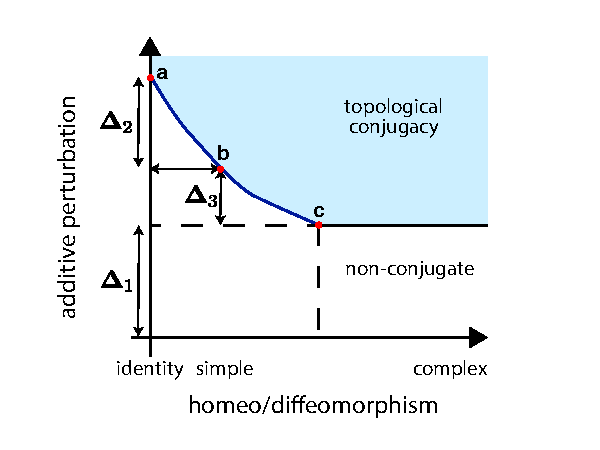
\includegraphics{pareto}
\caption{The two measures of distortion to map the source system to the target system forms a Pareto frontier boundary. See.~\eqref{eq:decomp:triple} for the symbols.}
\label{fig:pareto}
\end{figure}

\subsection{Integrated bound}
The bound \eqref{eq:h:bound} holds point-wise.
Given a distribution over trajectories (orbits of finite duration),
$p(\phi(\vx_0,T_\text{max}))$, we can integrate the inequality over the marginal probability measure $p(\vx)$:
\begin{align}\label{eq:h:bound:integrated}
    \E_\vx \norm{\vDelta(\vx)}
    &\leq
	\E_\vx
	\left[
	    \norm{\vf(\vx)}
	    \cdot
	    \norm{\nabla\tilde\homeo(\vx)}
	\right]
	+
	\E_\vx
	\left[
	    \norm{\nabla\vf(\vx)}
	    \cdot
	    \norm{\tilde\homeo(\vx)}
	\right]
	+ O(\epsilon)
\end{align}

\subsection{Divergence}
We are ready to define the divergence measure between the source and target systems under the probability distribution over states.
\begin{align}\label{eq:divergence}
    \IMPdivv{\vf}{\vg}{\mu}
	&\coloneqq
	\left(
	\inf_\Delta
	,
	\inf_\homeo
	\right)
\end{align}

\bibliographystyle{unsrtnat_IMP_v1}
\bibliography{../all_ref.bib,imprefs,../catniplab.bib}
\end{document}
